\documentclass[12pt]{article}
\usepackage[russian]{babel}
\usepackage[utf8]{inputenc}
\usepackage{amssymb}
\usepackage{amsmath}
\usepackage{latexsym}
\usepackage{enumitem}
\usepackage[margin=1.5cm]{geometry}
\usepackage{relsize}
\usepackage[thinlines]{easytable}
\usepackage{mathrsfs}
\usepackage{graphicx}
\usepackage{wrapfig}
\usepackage{multicol}

\newcommand{\rchoose}[2]{\left(\mkern-6mu \left({#1 \atop #2}\right) \mkern-6mu \right)}
\newcommand{\dsum}{\sum_{\substack{ k\le n \\ k - \text{нечетное}}}}
\renewcommand{\P}{\text{Pr}}
\newcommand{\eps}{\varepsilon}
\newcommand{\dto}{\Rightarrow}
\newcommand{\none}{$\varnothing$}

\begin{document}

\title{Формальные грамматики \\ Домашняя работа 2}
\author{Антон Афанасьев}
\maketitle
\begin{enumerate}
	\item[1.]
	\begin{multicols}{2}
	Грамматика в нормальном виде Хомского для языка Дика и таблица разбора строки $abaabba$.\\ \\
	$S \to AC \mid DD \mid \eps$ \\
	$C \to DB \mid b$ \\
	$D \to AC \mid DD$ \\
	$A \to a$ \\
	$B \to b$

\columnbreak
\begin{TAB}(e,0.5cm,2cm){|c|c|c|c|c|c|c|c|c|}{|c|c|c|c|c|c|c|c|}
  & 0 & 1 &   2  & 3     & 4     & 5     & 6     & 7     \\
0 &   & A & S, D & \none & \none & \none & S, D  & \none \\
1 &   &   & B, C & \none & \none & \none & \none & \none \\ 
2 &   &   &      & A     & \none & \none & S, D  & \none \\ 
3 &   &   &      &       & A     & S, D  & C     & \none \\ 
4 &   &   &      &       &       & B, C  & \none & \none \\ 
5 &   &   &      &       &       &       & B, C  & \none \\ 
6 &   &   &      &       &       &       &       & A     \\ 
\end{TAB}
\end{multicols}
	\item[2.] Разбор алгоритмом Валианта.
	Изменение ячейки $P_{0, 6}$ произойдет при вызове процедуры \linebreak $complete(0, 4, 4, 8)$. К этому моменту будут подсчитаны значения T в области отмеченной на рисунке серым. Процедура complete сначала посчитает подматрицы $\mathscr{D, C, D'}$ (при этом подматрица $\mathscr{E}$ содержащая ячейку $(0, 6)$ затронута не будет). \\
	$P_{0, 6}$ изменится при выполнении действия $P_{\mathscr{E}} = P_{\mathscr{E}} \cup (T_{\mathscr{B}} \times T_{\mathscr{D'}})$. После этого действия в ячейке $P_{0, 6}$ окажется пара нетерминалов (D, D), что сделает условие $S \in f(P_{0, 6})$ верным. В терминах булевых матриц это произойдет когда будут перемножаться две подматрицы хранящие логические значения ``можно ли породить подстроку нетерминалом D'':
	
	\begin{multicols}{2}
	$\underset{\mathlarger{T^D_{\mathscr{B}}}}{\begin{pmatrix} 1 & 0 \\ 0 & 0 \end{pmatrix}} \times \underset{\mathlarger{T^D_{\mathscr{D'}}}}{\begin{pmatrix} 1 & 0 \\ 0 & 0 \end{pmatrix}} = \underset{\mathlarger{P^{DD}_{\mathscr{E}}}}{\begin{pmatrix} 1 & 0 \\ 0 & 0 \end{pmatrix}}$
	
	\columnbreak
	
    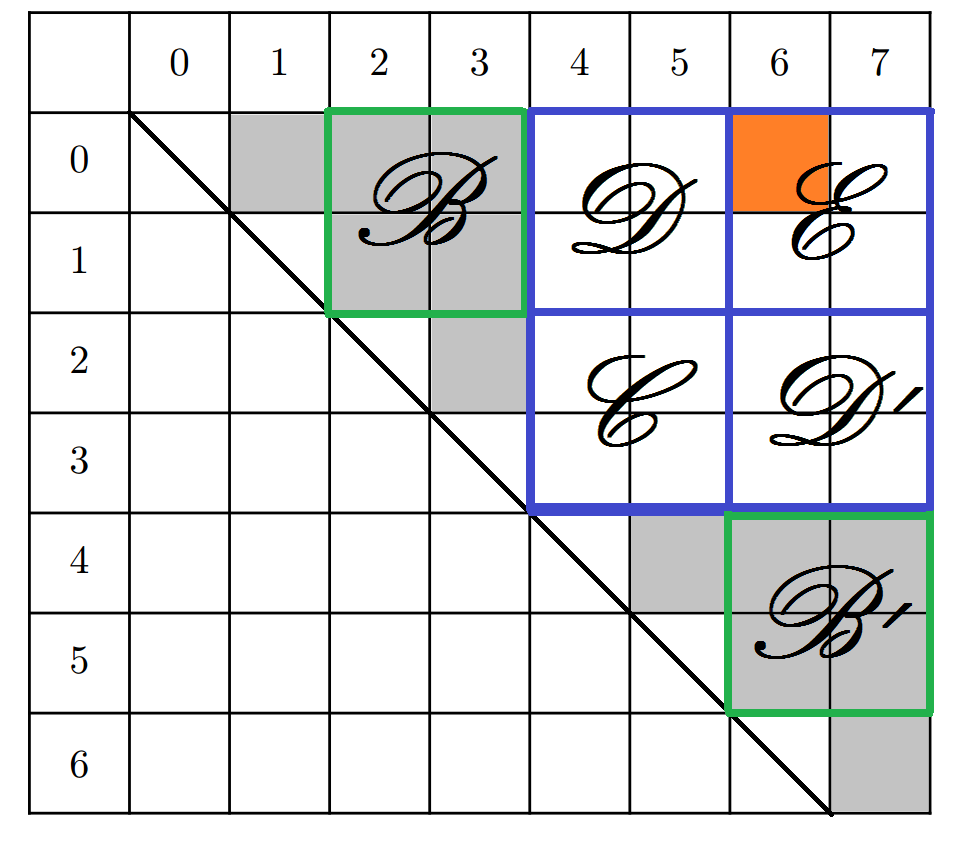
\includegraphics[width=0.4\textwidth]{valiant}
	\end{multicols}
	\item[3.] Возьмем язык $L_1 = \left \{ a^n \{b, c\}^n \mid n \ge 0 \right\}$. Этот язык LL(1), так как порождается следующей LL(1) грамматикой:
	
	$S \to aSD \mid  \eps$\\
	$D \to b \mid c$
	
	Возьмем также регулярный язык $L_R = a^*b^* \cup a^*c^*$.
	
	Рассмотрим пересечение этих языков $$L_2 = L_1 \cap L_R = \left \{ a^n b^n \mid n \ge 0 \right \} \cup \left \{ a^n c^n \mid n \ge 0 \right \}$$
	Про язык $L_2$ известно, что он не LL(k), следовательно, класс LL не замкнут по пересечению с регулярными языками.
	
	\item[4.] Линейная грамматика для NLOGSPACE-полного языка.
	
	$S \to [F]$ \\
	$F \to M \mid Z \mid X$ \\
	$Z \to Za \mid Zb \mid Z \$ \mid F\#$ \\
	$X \to aX \mid bX \mid \$ X \mid \# F$ \\
	$M \to aMa \mid bMb \mid \$ \mid T\# \mid \#Q \mid \  ][D \mid E][$\\
	$T \to Ta \mid Tb \mid T\$ \mid T\# \mid E][$\\
	$E \to M \mid B$ \\
	$B \to Ba \mid Bb \mid B\$ \mid E\#$ \\
	$Q \to aQ \mid bQ \mid \$Q \mid \#Q \mid \ ][D$ \\
	$D \to M \mid A$ \\
	$A \to aA \mid bA \mid \$A \mid \#D$
	
	\item[5.] По обыкновенной грамматике определить, порождает ли она хотя бы одну строку четной длины. Эта задача разрешима, приведем алгоритм. \\
	Приведем грамматику в нормальную форму Хомского. Заведем два множества ODD и EVEN. Будем помещать нетерминал в множество ODD если он может породить строку нечетной длины, а в множество EVEN если нетерминал может породить строку четной длины. Изначально оба множества пусты. \\
	Для всех правил вида $A \to a$ добавим A в множество ODD. Если есть правило $S \to \eps$, то добавим S в множество EVEN. \\
	Далее, для каждого правила $A \to BC$ будем действовать следующим образом
	\begin{itemize}
		\item $(B \in ODD \land C \in ODD) \dto EVEN = EVEN \cup \{A\}$
		\item $(B \in EVEN \land C \in ODD) \dto ODD = ODD \cup \{A\}$
		\item $(B \in ODD \land C \in EVEN) \dto ODD = ODD \cup \{A\}$
		\item $(B \in EVEN \land C \in EVEN) \dto EVEN = EVEN \cup \{A\}$
	\end{itemize}
	
	Будем продолжать это делать до тех пор, пока множества не перестанут меняться. Так как мы только добавляем элементы в множества, то этот процесс когда-нибудь остановится (т.к. число нетерминалов конечно). Легко видеть, что теперь множества ODD и EVEN заполнены корректно. Ответ на задачу (порождает ли грамматика строку четной длины) эквивалентен вопросу принадлежит ли стартовый нетерминал множеству EVEN.
	
	\pagebreak
	
	\item[6.] По обыкновенной грамматике определить, порождает ли она хотя бы одну строку-палиндром. Эта задача неразрешима. Покажем это, сведя к ней задачу на проверку непустоты пересечения языков порождаемых обыкновенными грамматиками.
	
	Возьмем две грамматики $G_1$ и $G_2$. Обозначим языки которые они порождают $L_1 = L(G_1)$ $L_2 = L(G_2)$. Пусть символ $\#$ не входит в алфавиты $L_1$ и $L_2$. 
	
	Рассмотрим язык $L_0 = L_1 \cdot \{\#\} \cdot L^R_{2}$ --- конкатенация строк первого языка с перевернутыми словами второго языка через решетку. Так как обыкновенные языки замкнуты по конкатенации и по перевороту, то для этого языка существует обыкновенная грамматика $G_0$. (Замкнутость по операции переворота по моему на лекциях не обсуждалось, но ясно, что для получения дерева разбора для перевернутой строки достаточно отразить по вертикали дерево разбора для исходной строки, а для того чтобы всегда получать такие перевернутые деревья разбора достаточно перевернуть все правые части правил)
	
	Теперь, если $L_1 \cap L_2 \neq \varnothing$, то $\exists w\ w \in L_1, w \in L_2$ и $w\#w^R \in L_0$ то есть язык $L_0$ содержит палиндром. \\
	В обратную сторону, если $L_0$ содержит палиндром, то так как все строки в нем вида $a\#b^R$, причем $a \in L_1,\ b \in L_2$, то палиндром имеет вид $w\#w^R$. А это значит, что $w \in L_1,\ w \in L_2$ и $L_1 \cap L_2 \neq \varnothing$.
	
	Таким образом $L_1 \cap L_2 \neq \varnothing$ тогда и только тогда, когда $L_0$ содержит палиндром. Следовательно, если мы сможем ответить на вопрос ``по грамматике $G_0$ сказать порождает ли она палиндром'', то мы сможем сказать пусто или нет пересечение $L_1$ и $L_2$. Так как последняя задача неразрешима, то и задача проверки на порождение палиндрома тоже неразрешима.

	\item[7.] Будем действовать следующим образом: запустим алгоритм распознающий строку для всех циклических сдвигов входной строки. Возьмем алгоритм 10.1 из 14 лекции, распознающий обычные языки за $O((\log n)^2)$ памяти. Для того чтобы не использовать лишней памяти на хранение подстрок параметризуем алгоритм текущим сдвигом $\mathit{offset}$, и в том месте где идет обращение к символам входной строки будем обращаться не по индексу $j$, а по индексу $1 + ((j + \mathit{offset}-1) \!\! \mod n)$ где $n$ - длина строки, а mod --- взятие остатка от деления. Таким образом работа алгоритма ничем не будет отличаться от работы на циклически сдвинутой строке.
	
	Запустим алгоритм для всех циклических сдвигов, и если хотя бы один из них принадлежит языку, то ответить ``да''. Так как никакой памяти, кроме используемой алгоритмом разбора из лекции, мы не использовали, то требуемый объем памяти $O((\log n)^2)$.
\end{enumerate}
\end{document}
